\newpage
\hypertarget{M2TSettingUp tex}{}
\subsection{Initializing the project}
\texHeader

{\bf SELF:: update download so it includes a constraint file for \texttt{Dictionary}}
\begin{figure}[htbp]
\begin{center}
  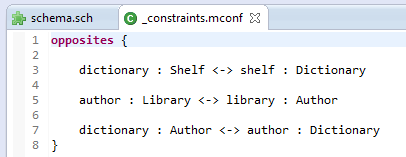
\includegraphics[width=0.7\textwidth]{eclipse_DOWNLOADUPDATE}
  \caption{SELF SELF}
\end{center}
\end{figure}

\begin{enumerate}

\item[$\blacktriangleright$] Your expanded \texttt{DictionaryLanguage} metamodel MOSL structure should resemble FIG. (starting point) You'll notice that it is
accessing the \emph{Moca} framework by importing the \texttt{MocaTree} in \texttt{\_imports.mconf}. (Explain, no screenshot?)

\item[$\blacktriangleright$] Right click on \texttt{MyWorkingSet} folder and create a new TGG. source: MocaTree. Target: DictionaryLanguage. FIG

\begin{figure}[htbp]
\begin{center}
  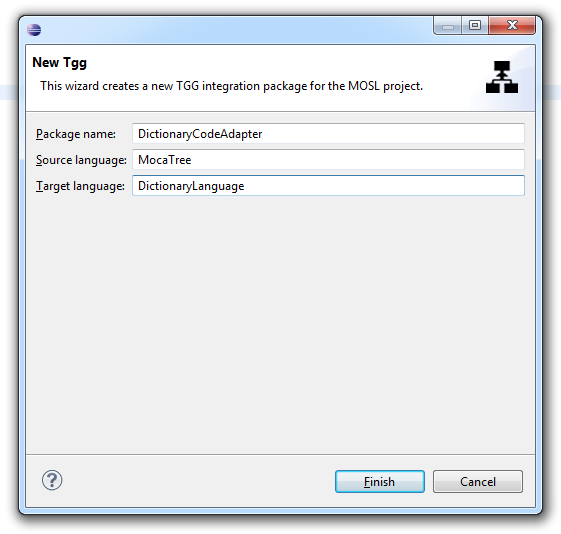
\includegraphics[width=0.9\textwidth]{eclipse_dictionaryCodeAdapterTGGProject}
  \caption{create tgg}
  \label{eclipse:newTGGProject}
\end{center}
\end{figure}


\item[$\blacktriangleright$] Before saving and building, initialize the correct generated code type by establishing the schema below (default is..)

\begin{figure}[htbp]
\begin{center}
  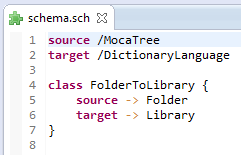
\includegraphics[width=0.5\textwidth]{eclipse_schemaStart}
  \caption{first rule}
  \label{eclipse:firstSchema}
\end{center}
\end{figure}

\item[$\blacktriangleright$] Save and build your project! Confirm a generated project was created in the \texttt{MyWorkingSet} node, and carry on!

\end{enumerate}
